% -*- coding: utf-8 -*-

\ifx\firstpassage\undefined
\def\firstpassage{1}
\newcount\nbpassages
\nbpassages=1



\documentclass[10pt,onecolumn]{article}

\usepackage{ucs}
%\usepackage[utf8x]{inputenc}
%\usepackage{CJK}
\usepackage[T1]{fontenc}
\usepackage{amsmath}
\usepackage{amssymb}
\usepackage{subfigure}
\usepackage{float}
\usepackage{latexsym}
\usepackage{amsfonts}
\usepackage{epic}
\usepackage{eepic}
\usepackage{makeidx}
\usepackage{multido}
\usepackage{varindex}
\usepackage{moreverb}
\usepackage[usenames]{color}
\usepackage{alltt}
\usepackage{moreverb}
\usepackage{fancyvrb}
\usepackage{fancyhdr}
\usepackage{color}
\usepackage{eurosym}
\usepackage{multirow}
\usepackage[small,normal]{caption2}  % hang
\usepackage{tabularx}
\usepackage{placeins}
\usepackage{hyperref}
\usepackage{url}
\urlstyle{sf}
\usepackage[lmargin=3cm,rmargin=3cm,tmargin=3cm,bmargin=3cm]{geometry}
\pagestyle{fancy}
\usepackage{xcolor}
\usepackage{colortbl,hhline}

\usepackage[pdftex]{graphicx}   %[pdftex]
\usepackage{mfpic}

\usepackage{lscape}
\usepackage{rotating}
\usepackage[all]{xy}

\newcommand{\pa}[1]						{ \left(#1\right)}
\newcommand{\cro}[1]						{ \left[#1\right]}
\newcommand{\acc}[1]					{ \left\{#1\right\}}
\newcommand{\ydirac}[1]				{ \mathbf{1\!\!1}_{\acc{#1}} }
\newcommand{\suggestion}[2] 	{\bigskip \textbf{Suggestion:}\\ \index{suggestion!#1}#2}
\newcommand{\moredetail}[2] 	{\bigskip \textbf{More details:}\\ \index{more details!#1}#2}
\newcommand{\murl}[1]					{\footnotesize{\url{#1}}\normalsize}
\newcommand{\infegal}[0]			{\leqslant}
\newcommand{\supegal}[0]			{\geqslant}
\newcommand{\abs}[1]						{ \left|#1\right|}
\newcommand{\turl}[1]{\begin{scriptsize}\url{#1}\end{scriptsize}}
\newcommand{\indicatrice}[1]{\mathbf{1\!\!1}_{\acc{#1}}}
\newcommand{\pr}[1]						{\mathbb{P}\pa{#1}}

\parindent 0pt

\newcommand{\firstpassagedo}[1]{ \ifnum\nbpassages=1 #1 \fi }

\sloppy

% graphics part
\setlength{\unitlength}{1cm}

% rectangle x,y,w,l
\newcommand{\figrect}[4]			{ \multiput(#1, #2)(#3, 0){2}{\line(0, 1){#4}}
																\multiput(#1, #2)(0, #4){2}{\line(1, 0){#3}} }
\newcommand{\figrecttext}[5]	{ \multiput(#1, #2)(#3, 0){2}{\line(0, 1){#4}}
																\multiput(#1, #2)(0, #4){2}{\line(1, 0){#3}} 
																\put(#1,#2){#5}}


\newenvironment{mbpicture}[2] 	{  \begin{center} \begin{tabular}{|c|} \hline \\  \begin{minipage}{#1 cm} \begin{picture}(#1,#2) }
															{ \end{picture} \end{minipage}  \\ \hline \end{tabular}\end{center}  }

\newenvironment{ypicture}[2] 	{  \begin{center} \begin{picture}(#1,#2) }
													 		{ \end{picture} \end{center}}
													 		

\makeindex

\newcounter{xcremark}[section]
\renewcommand{\thexcremark}    {\thesection.\arabic{xcremark}}

\newenvironment{remark}[1] 	{\refstepcounter{xcremark}\medskip\textbf{Remark \thexcremark: #1}\index{remark!#1}\\}
													 	{ }

\newcommand{\cpp}[0]{\textit{C++}}
\newcommand{\cpps}[0]{\textit{C++} }

\newcommand{\codes}[1]{\small$\mathtt{#1}$\normalsize}
\newcommand{\codesnote}[1]{$\mathtt{#1}$}

\if 1
\makeatletter  % makes '@' an ordinary character
\renewcommand{\verbatim@font}{%
\ttfamily\small%
\catcode`\^^I=\active \gdef^^I{\ \ \ \ }%
\catcode`\`=\active\gdef`{\relax\lq}%
\catcode`\<=\active\catcode`\>=\active%
\catcode`\^^I=\active%
\catcode`\<=\active \catcode`\>=\active %
\catcode`\,=\active \catcode`\'=\active %
\catcode`\`=\active%
}
\makeatother   % makes '@' a special symbol again
\fi


\DefineVerbatimEnvironment{verbatimx}{Verbatim}{%
frame=single, framerule=.1pt, framesep=1.5mm, fontsize=\footnotesize,
%gobble=2,
%fillcolor=\color{yellow},
xleftmargin=0pt
}

\setlength{\parskip}{1ex plus 0.5ex minus 0.2ex}

\newcommand{\definespacepar}[0]{ \setlength{\parskip}{1ex plus 0.5ex minus 0.2ex} }
\newcommand{\citeindex}[1]{}
\newcommand{\indexfr}[1]{}
\newcommand{\indexfrr}[2]{}


%\setlength{\topsep}{0pt}
%\setlength{\partosep}{0pt}
%\setlength{\itemsep}{0pt}

\newenvironment{myitem}%
{ \begin{list}%
	{$\bullet$}%
	{\setlength{\labelwidth}{30pt}%
	 \setlength{\leftmargin}{35pt}%
	 \setlength{\parskip}{0pt}
	 \setlength{\itemsep}{0pt}
	 \setlength{\parsep}{0pt}
	 }}%
{ \end{list} }

\newcommand{\inputcode}[2]{\index{program!#2}
 %\VerbatimInput[frame=single,numbers=right,numbersep=2pt,stepnumber=5,firstnumber=1,fontsize=\footnotesize]{#1} }
\VerbatimInput[frame=single,fontsize=\footnotesize]{#1} }


\newcommand{\nsubset}[0]{\subset \hspace{-9pt} \backslash \hspace{4pt} }

\rfoot[paire droite]{\begin{footnotesize} \textit{\date{\today}} \end{footnotesize}}
\lfoot[paire droite]{\begin{footnotesize} \textit{Microsoft STC Europe%Confidential
																									} \end{footnotesize}}
\newcommand{\msn}[0]{\textit{Microsoft}}
\newcommand{\msns}[0]{\textit{Microsoft }}

\hyphenation{digging}
\hyphenation{selecting}

%\include {../_header_footer/ideogram.tex}
\newcommand{\unicode}[1]{\includegraphics{../_ideogram/char_0x#1.png}}
\newcommand{\unicodes}[1]{\includegraphics[height=0.6cm]{../_ideogram/char_0x#1.png}}

\begin{document}


\else


\ifnum\nbpassages=3
\nbpassages=4
\fi

\ifnum\nbpassages=2
\nbpassages=3
\fi

\ifnum\nbpassages=1
\nbpassages=2
\fi

\fi


\ifnum\nbpassages=1
\title{Precision, Recall, DCG}
\author{Xavier Dupre}
\date{\today}
\maketitle
\setcounter{tocdepth}{3}

\tableofcontents

\definespacepar
\bigskip
\fi

\section{Precision, Recall}

Let's consider a query classifier which aims at determining the language of a query. It can be seen as a function which takes query~$q$ and returns a country code and a score. The score reflects the confidence the function has in its result. Next table gives some examples of the expected behaviour of such a function:

\begin{center}\begin{tabular}{|l|c|r||r|}\hline
\textbf{query} & \textbf{country code} & \textbf{score} & \textbf{correct} \\ \hline
the financial crisis & en & 0.90 & true \\ 
la crise financiere & fr & 0.85 & true \\
izquierda derecha & es & 0.95 & true \\
toilettes  & fr & 0.75 & true \\
pull over & fr & 0.45 & false \\
sarkozy & hu & 0.80 & false \\
elephant gris & en & 0.65 & false \\
pork epic & en & 0.75 & false \\
impossible & fr & 0.30 & true \\ \hline
\end{tabular}\end{center}

The score gives an information about the confidence of the function. We could use it to determine whether taking a decision is relevant or not. Let's consider the classifier is doing a good job when its score is above~0.70. Next table gives an overview of the results:

\begin{center}\begin{tabular}{|l|c|r||r||l|}\hline
\textbf{query} & \textbf{country code} & \textbf{accepted} & \textbf{correct} & \textbf{class} \\ \hline
the financial crisis & en & 1 & 1 & TP\\ 
la crise financiere & fr & 1 & 1  & TP\\
izquierda derecha & es & 1 & 1  & TP\\
toilettes  & fr & 1 & 1& TP \\
pull over & fr & 0 & 0 & FN\\
sarkozy & hu & 1 & 0  & FP \\
elephant gris & en & 0 & 0 & FN \\
pork epic & en & 1 & 0 & FP  \\
impossible & fr & 0 & 1 & TN\\ \hline
\end{tabular}\end{center}

Each query then belong to one the four following categories\footnote{See also \murl{http://en.wikipedia.org/wiki/Precision\_and\_recall}.}:

\begin{center}\begin{tabular}{|l|l|}\hline
TP: True, Positive & FP: False, Positive  \\ \hline
FN: True, Negative & TN: False, Negative \\ \hline
\end{tabular}\end{center}

\begin{enumerate}
\item TP: the score is high enough, the answer is accepted and the answer is good
\item FP: the score is high enough, the answer is accepted but the answer is false
\item FN: the score is not high enough, the answer is rejected but the answer is true
\item TN: the score is not high enough, the answer is rejected and the answer is false
\end{enumerate}

In our case, it gives:
\begin{center}\begin{tabular}{|r|r|}\hline
4  &  1 \\ \hline
1 & 2 \\ \hline
\end{tabular}\end{center}

At this point, we can define the precision and the recall for this threshold:

\begin{eqnarray}
precision &=& \frac{ TP } { TP + FP } = \frac{4}{4+2} = 66\%\\
recall &=& \frac{ TP } { TP + FN } = \frac{4}{4+1} = 80\%
\end{eqnarray}

If we change the score, these two ratios are different. We can draw the two ratios on the same graph against the threshold (see Figure~\ref{figure_precision_recall_threshold}).

\begin{figure}[ht]
\begin{center}\begin{tabular}{|c|} \hline
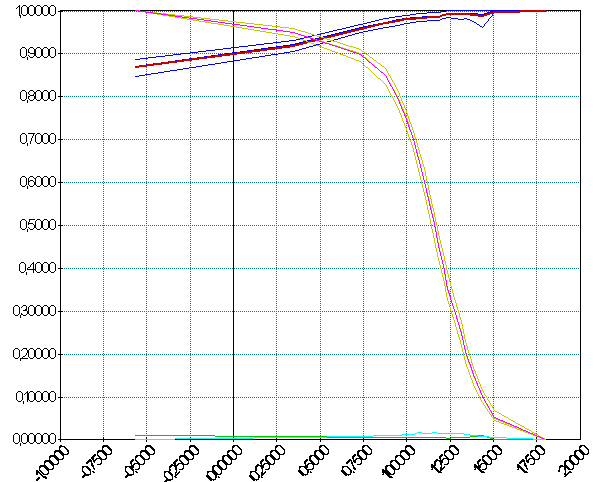
\includegraphics[width=6cm]{image/prerecall.png} \\ \hline
\end{tabular}\end{center}
\caption{Precision and Recall against the threshold. X-Axis: threshold, Y-Axis: precision and recall.}
\label{figure_precision_recall_threshold}
\end{figure}


It is not easy to determine the best threshold, it depends on the constraints. We could try to maximize a kind of average:

\begin{eqnarray}
f_{\beta} &=& \frac{ (1+\beta^2) P R} { \beta^2 P + R}
\end{eqnarray}

$P$ stands for precision and $R$ for recall. We usually use $\beta=1$ which is similar to a geometric average.

\section{AUC or Area Under the Curve}

We usually find another way to represent a curve precision-recall. We need the score to compute the two ratios but it has no meaning. The curve ROC (Receiving Operator Characteristic\footnote{See also~\murl{http://en.wikipedia.org/wiki/Receiver\_operating\_characteristic}.}) represents the precision against the recall. Each point on this curve (see Figure~\ref{figure_roc}) was obtained with a specific score.


\begin{figure}[ht]
\begin{center}\begin{tabular}{|c|} \hline
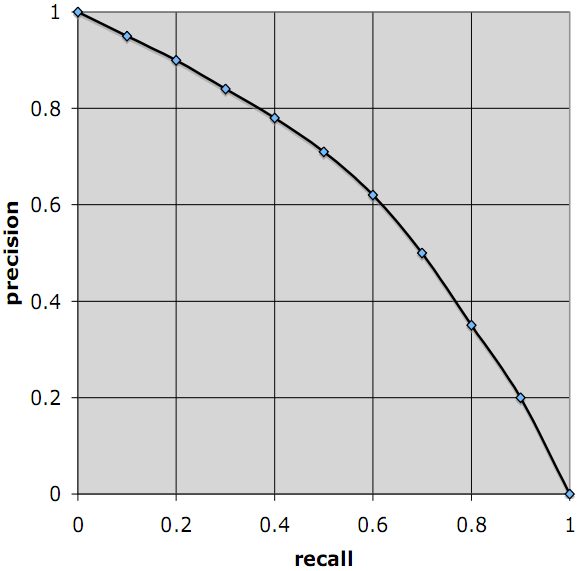
\includegraphics[width=6cm]{image/oneroc.png} \\ \hline
\end{tabular}\end{center}
\caption{ROC curve. The Area Under the Curve (AUC) is one indicator of the accuracy of the classifier. A straight line between point (0,1) and (1,0) indicates a random classifier. Above this line, the classifier performs better than random. }
\label{figure_roc}
\end{figure}



We call AUC the Area Under the Curve. If we consider all the examples $(x_1,...,x_p)$ for which the function takes a good decision and all the examples for which the function takes the wxrong decision $(y_1,...,y_q)$. We can demonstrate that:

\begin{eqnarray}
AUC = \frac{ \sum_{i,j} \indicatrice{x_i \supegal y_j} }{ pq }
\end{eqnarray}

It is a way to compare two functions which classifies a query: the best classifier maximizes the AUC.

\section{Discounted Cumulative Gain (DCG)}

For every query, we consider the first five results. A human operator classifies each of them in five categorties\footnote{See also \murl{http://en.wikipedia.org/wiki/Discounted\_Cumulative\_Gain}.}:

\begin{enumerate}
\item P for Perfect: there is no better result, this one is expected
\item E for Excellent: it is a good result
\item G for Good: it is a result related to the query
\item F for Fair: it does not bring any information
\item B for Bad: it confuses the uses
\end{enumerate}

We give to every category a weight:

\begin{center}\begin{tabular}{ccccc}
P & E & G & F & B \\
10 & 7 & 3 & 0.5 & 0
\end{tabular}\end{center}

We also give a weight to every position because it is better to have a perfect result in the first position rather than in the fifth one. Let's denote the judgment for result $r_i$ in position~$i$, we define the DCG(5) for the first five result as:

\begin{eqnarray}
DCG(5) = \sum_{i=1}^{5} \frac{ r_i } { \ln_2 (1+i) }
\end{eqnarray}

This figure takes into account the relevance and the order of the result. The $nDCG$ only takes into account the order. We define:

\begin{eqnarray}
DCG^*(5) = \sum_{i=1}^{5} \frac{ r_{\sigma(i)} } {\ln_2 (1+i) }
\end{eqnarray}

Where $r_{\sigma(1)} \supegal r_{\sigma(2)} \supegal ... \supegal r_{\sigma(5)}$. It means we change the position of results in order to get the most relevant ones in the first positions. Then: 

\begin{eqnarray}
nDCG(5) =  \frac{ DCG(5) } { DCG^*(5) }
\end{eqnarray}

The DCG is not the only way to measure a search engine accuracy. It does not take into account a same perfect could appear twice. Two perfect results would artificially increase the DCG\footnote{See also~\ref{http://learningtorankchallenge.yahoo.com/instructions.php}, or \murl{http://olivier.chapelle.cc/pub/err.pdf}.}. The full evaluation of a search engine requires a random sample of queries to get the average DCG(5). In order to get a confidence interval, we could draw another random set of queries but the evaluation of each results requires time. It is also possible to bootstrap\footnote{See \murl{http://en.wikipedia.org/wiki/Bootstrapping\_(statistics)}.}.


\section{Precision, Recall for DCG}

Defining the recall of a search engine is impossible unless we can evaluate every url as a result of a specific query. There are two many pairs. We then try to define a limited recall measured while we compare two search engine such as Google and Bing. For a query~$q$, we know the five results from Google and the five ones from Bing. We can then merge them into a single list and order them by decreasing order: it is the golden list built on Bing and Google result. For every search engine, we can define a $DCG(5)$. By merging the results from both engines, we could also build the golden list for this query which would have a $DCG^{**}(5)$. In this case, we may consider as a precision and a recall the following ratios:

\begin{eqnarray}
precision(Bing) &=& \frac{DCG_{Bing}(5)}{DCG^*_{Bing}(5)}\\
recall(Bing)    &=& \frac{DCG_{Bing}(5)}{DCG^{**}(5)} 
\end{eqnarray}

The same formula can be applied For several queries, we would have:
\begin{eqnarray}
precision(Bing) &=& \frac{\sum_q DCG_{Bing}(5)}{\sum_q DCG^*_{Bing}(5)}\\
recall(Bing)    &=& \frac{\sum_q DCG_{Bing}(5)}{\sum_q DCG^{**}(5)} 
\end{eqnarray}

The same figures can be computed for Google. This is not the only to measure the precision recall. For a query~$q$, we now define $g(q,p,r) \in {0,1}$, it is~1 if Google gives a results whose relevance is greater than~$r$ before position~$p$. We define the same way $b(q,p,r)$ for Bing, and $f(q,p,r)$ for the golden set. The precision and recall in this case are defined by:

\begin{eqnarray}
precision(Bing) &=& \frac{\sum_q b(q,p,r)}{\sum_q b(q,\infty,r)}\\
recall(Bing)    &=& \frac{\sum_q b(q,p,r)}{\sum_q f(q,p,r)} 
\end{eqnarray}

There are many others ways to compare the performance of search engines\footnote{See also \murl{http://dasdan.net/ali/www2009/web-search-metrics-tutorial-www09-parts0-5.pdf}.}.









%\begin{flushleft}
%\printindex
%\end{flushleft}

\ifnum\nbpassages=1
\nbpassages=0
\fi

\ifnum\nbpassages=2
\nbpassages=1
\fi

\ifnum\nbpassages=3
\nbpassages=2
\fi

\ifnum\nbpassages=0
\end{document}
\fi


